\section{Round Robin scheduling}

\begin{quote}
	\textit{Round robin es un método para seleccionar todos los elementos en un grupo de manera equitativa y en un orden racional, normalmente comenzando por el primer elemento de la lista hasta llegar al último y empezando de nuevo desde el primer elemento.} 
	
	\textit{El nombre del algoritmo viene del principio de Round-Roubin conocido de otros campos, donde cada persona toma una parte de un algo compartido en cantidades parejas.}\footnote{Fuente: Wikipedia: La enciclopedia libre.}
	
\end{quote}
	
	El algoritmo utiliza un intervalo de tiempo llamado \emph{quantum} que define la cantidad de tiempo que una tarea permanece en el procesador. Éste suele implementarse mediante un temporizador que genera una interrupción cuando se agota el tiempo.
	
	Las tareas se disponen en una cola simulando una estructura circular; la organización de la misma es \emph{FIFO}. Si una tarea agota su tiempo de procesamiento antes de finalizar el \emph{quantum}, ésta es desalojada y en su lugar se asigna otra tarea.
	
	Vale destacar que este algoritmo, si bien tiene un tiempo de espera grande, garantiza un reparto equitativo del procesador entre todas las tareas, lo cual lo hace libre de inanición.

\subsection{Implementación propuesta}

Nuestra implementación del \emph{scheduler} contiene tres métodos: \emph{load(pid)}, \emph{unblock(pid)} y \emph{tick(motivo)}, además de una cola para los procesos:

\begin{itemize}
	\item El método \emph{load(pid)} introduce una tarea con identificador \emph{pid} en la cola de tareas.
	
	\item El método \emph{unblock(pid)} avisa al \emph{scheduler} cuando la tarea con identificador \emph{pid} deja de estar bloqueada introduciéndola en la cola de tareas.
	
	\item El método \emph{tick(motivo)} se ejecuta por cada \emph{tick} del reloj de la máquina. El parámetro \emph{motivo} indica lo que ocurrió con la tarea que ocupaba el procesador el ciclo de reloj anterior:
	
	\begin{itemize}
		\item Si el \textbf{motivo} es \emph{block} o \emph{exit}: se reinicializa el \emph{quantum} y se saca la tarea de la cola. Cuando esto sucede y la cola queda vacía, se devuelve \verb|idle_task| ; de lo contrario el \emph{pid} de la tarea que ocupará el próximo ciclo de reloj.

		\item Si el \textbf{motivo} es \emph{tick}: si la tarea no era \verb|idle_task| y su \textit{quantum} finalizó, se devuelve el \emph{pid} de la tarea siguiente en la cola. Si todavía le queda tiempo para procesar, el \emph{pid} de la tarea que se procesó es el mismo que se retorna.
		
		Si la tarea era \verb|idle_task| y la cola está vacía, entonces continúa ejecutándose la misma tarea; de lo contrario se devuelve el \emph{pid} de la primer tarea de la cola y se reinicializa el \emph{quantum}.
	\end{itemize}

\end{itemize}

\subsection{Diagrama de estados}

\begin{figure}[H]
\centering
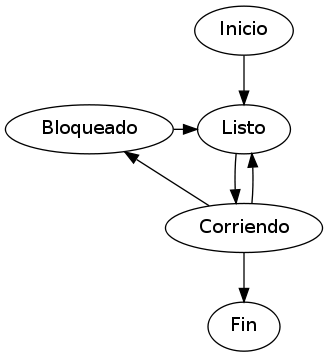
\includegraphics[scale=0.5]{estados.png}
\caption{En este diagrama de estados podemos apreciar el desalojo de tareas.}
\end{figure}

\subsection{Análisis del algoritmo}

Al realizar varias pruebas pudimos comprobar que a medida que aumentamos el \textit{quantum} haciéndolo proporcional al total de \emph{ticks} de las tareas, el tiempo necesario para que todas finalicen disminuye. Además podemos ver que el \emph{throughput} también mejora: a medida que el \emph{quantum} aumenta la proporción de tareas finalizadas por intervalo crece.

Esto es lo que podemos apreciar en los gráficos siguientes: las tareas, de tipo \verb|TaskBatch|, duran 10 \emph{ticks} y la cantidad de \emph{blocks} aumenta de 0 a 9. 

\begin{figure}[H]
\centering
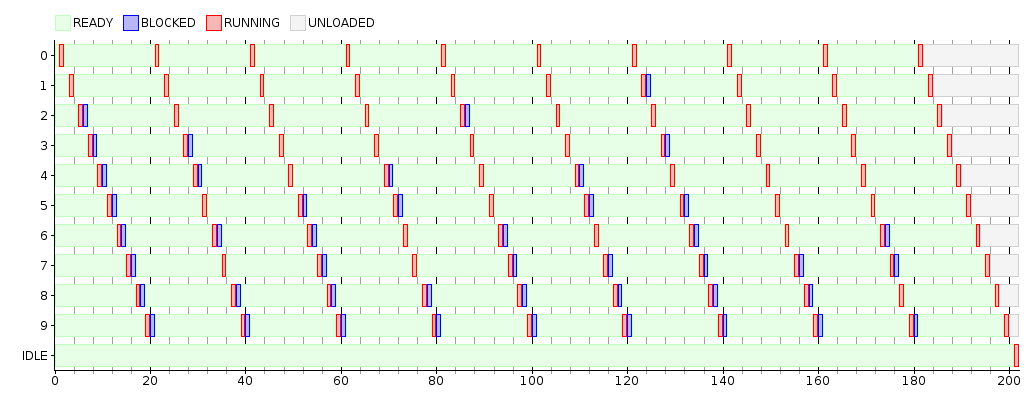
\includegraphics[scale=0.4]{./graficos/out_batch_fijo1.png}
\caption{Algoritmo \emph{Round Robin} con \emph{quantum} 1}
\end{figure}  

Como podemos apreciar este caso las tareas tardan alrededor de 200 \emph{ticks} de reloj en terminar. En cuanto al \emph{throughput} podemos ver que es bastante malo ya que todas las tareas terminan en un mismo intervalo, el último. 
 
\begin{figure}[H]
\centering
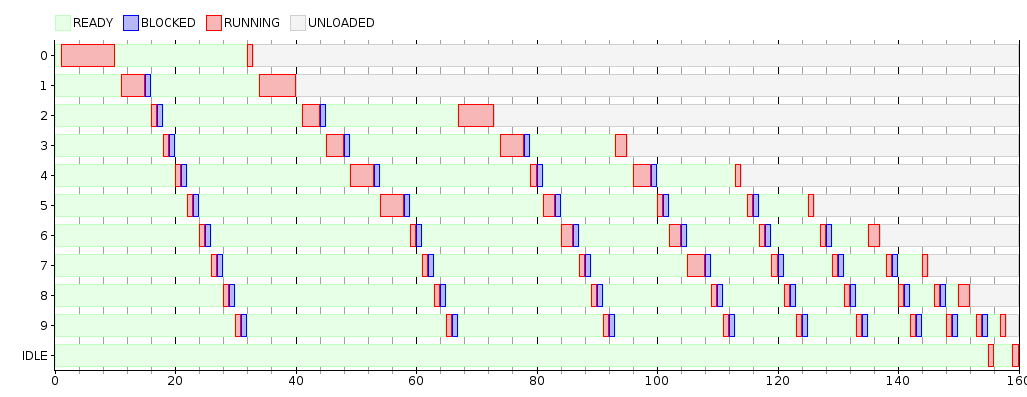
\includegraphics[scale=0.4]{./graficos/out_batch_fijo9.png}
\caption{Algoritmo \emph{Round Robin} con \textit{quantum} 9} 
\end{figure}

En este caso las tareas tardan alrededor de 160 \emph{ticks} de reloj en terminar y con respecto al \emph{throughput} vemos que mejora notablemente ya que la cantidad de tareas que finalizan por intervalo es mas uniforme.